\documentclass[11pt]{article}
\usepackage{fullpage}
\usepackage{graphicx}
\usepackage{longtable}
\usepackage{booktabs}
\usepackage{hyperref}

\providecommand{\tightlist}{%
  \setlength{\itemsep}{0pt}\setlength{\parskip}{0pt}}

\title{Design}
\date{}

\setlength\LTleft{0pt}
\setlength\LTright{0pt}

\setlength{\parskip}{\baselineskip}%
\setlength{\parindent}{0pt}%

\begin{document}
\maketitle
\tableofcontents
\newpage

\section{High-Level}\label{high-level}

The high-level design serves as a transition between the requirements
and the full low-level design. Below are designs used to identify key
components of the system and how they shall interact, both with each
other and with the user.

\subsection{Context Model}\label{context-model}

As with many computer games, this system is mostly `self-enclosed' -
that is, it does not require a large amount of interaction with
separately-developed external systems. Thus, the context of the Ant Game
system is minimal. However, unlike many other computer games, the style
of the game can require the user to provide some external `data' before
playing (an ant brain, and sometimes an ant-world). This means that
there is a possibility for external programs to be developed to aid the
user in writing a custom ant brain/world. This would mean that there
would be an interaction between the Ant Game program and two other
systems, as below:

\begin{center}
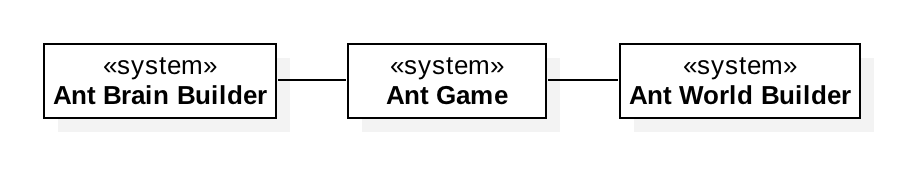
\includegraphics{diagrams/context-model.png}
\end{center}

However, as per the functional requirements document (\texttt{Game/4}
and \texttt{World/1}) the program shall parse ant brains and worlds from
a \emph{file} (i.e.~only indirectly received from outside software), so
this interaction with external programs does not need to be accounted
for in development.

\subsection{Process Model}\label{process-model}

\subsubsection{User Process}\label{user-process}

The process model on the following page describes a player interacting with the ant game
system. Note that the only two actions where the user is not directly
interacting with the program is the \texttt{Build\ Ant\ Brain} action
and \texttt{Build\ World} action - both of these actions are done
independently of this system by the user (in a text editor or
otherwise). This process model is abstract enough that it applies to
both the two-player game and the tournament. It is assumed that at least
two users are following this process model at the same time, and
interacting with the same instance of the program.

\begin{center}
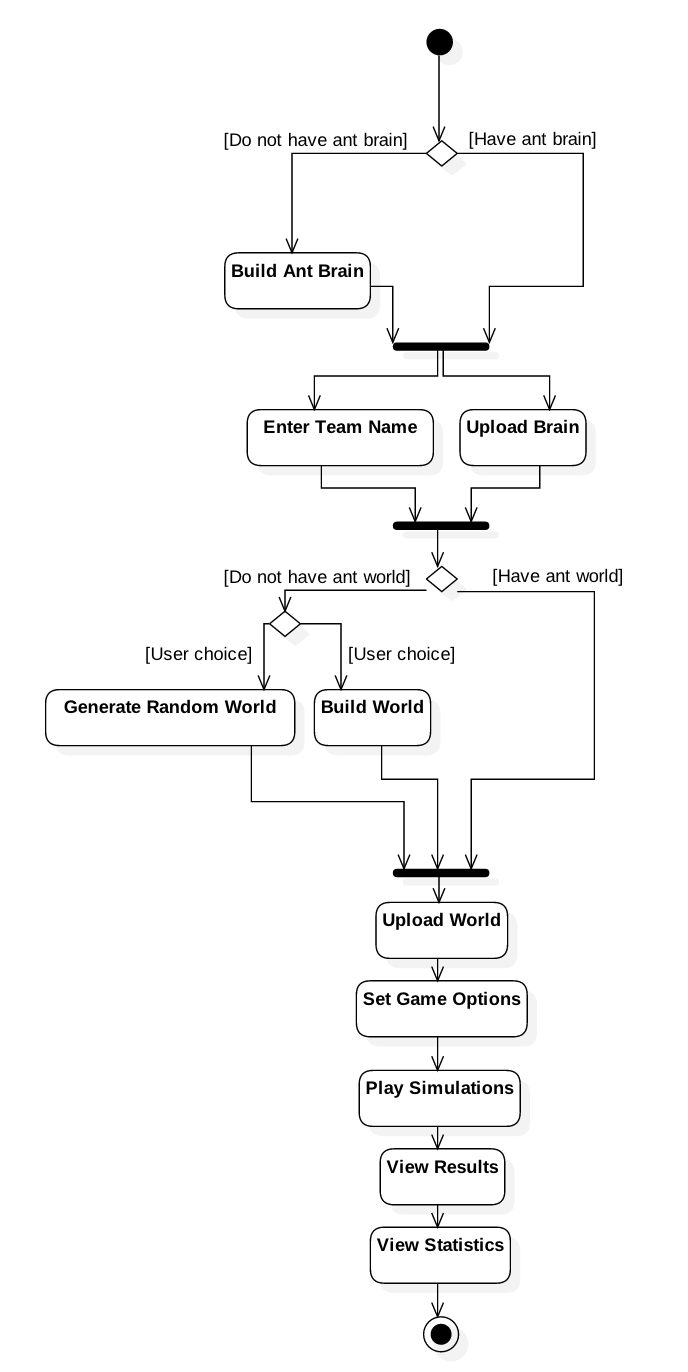
\includegraphics[width=\textwidth,height=\textheight,keepaspectratio]{diagrams/process-model.png}
\end{center}

\subsubsection{Game Process}\label{game-process}

The following diagram gives a high-level view of the flow of the system
when simulating a game between two ant colonies on a particular world.
Ant brains and a single world are loaded by two actors (the players).
The system then initialises ants on the two anthills for each colony.
Each ants identifiers are also initialised, as per the order in the
functional requirements. The game is then started, lasting for 300,000
rounds. Once the round counter is at its maximum, the food at each
anthill is counted; the team with the most food at their brains anthill
is declared the winner.

\begin{center}
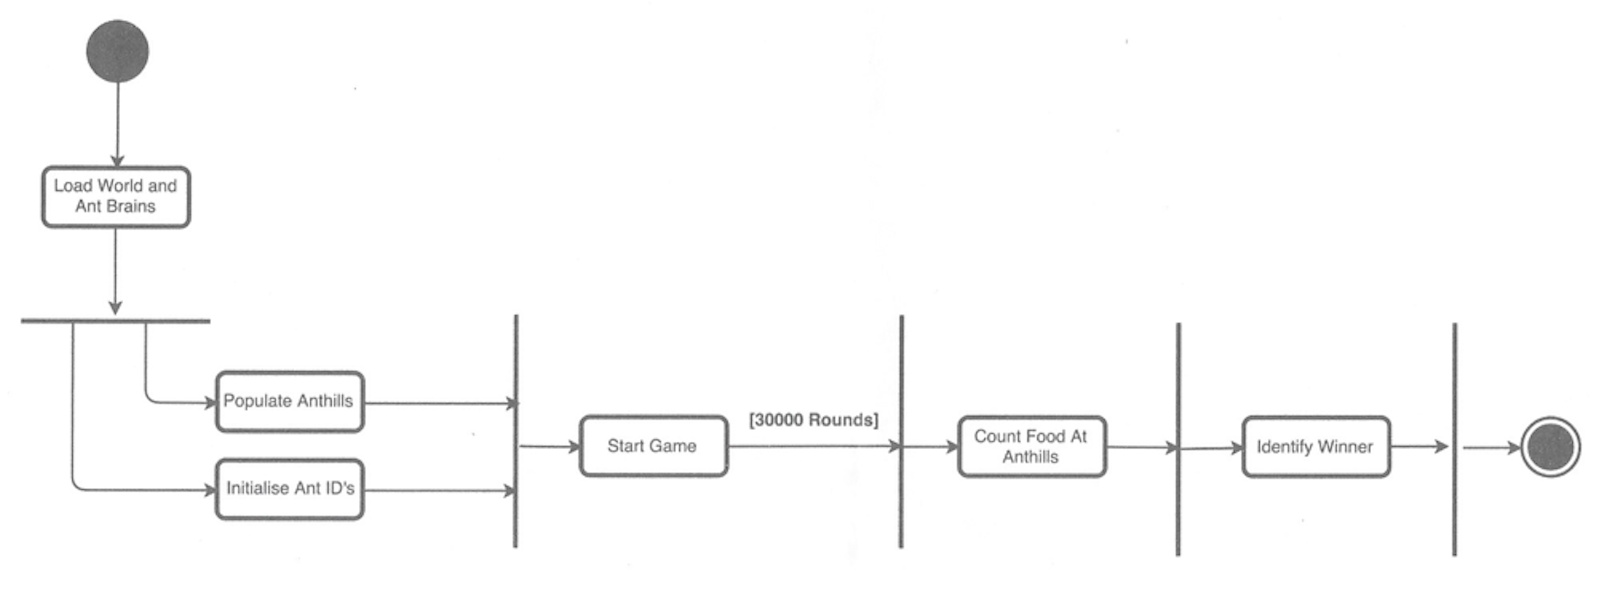
\includegraphics[width=\textwidth]{diagrams/process-model-game.png}
\end{center}

\subsection{Use Cases}\label{use-cases}

The process model makes it clearer as to how the user will interact with
the system. From the process model and the requirements, the primary use
cases of the system have been extracted, as below. The only (human)
actors in the following use cases are the players of the game.

\subsubsection{Upload Ant Brain}\label{upload-ant-brain}

\begin{center}
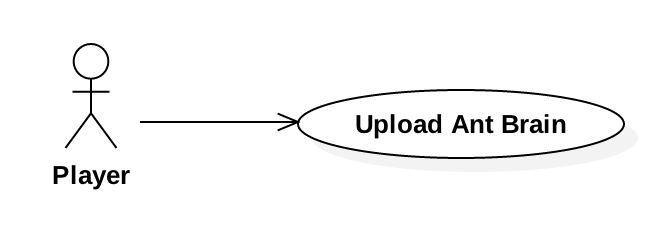
\includegraphics[width=0.4\textwidth]{diagrams/use-case-1-upload-ant-brain.png}
\end{center}

\begin{longtable}[c]{@{}p{0.2\textwidth}p{0.7\textwidth}@{}}
\toprule
& Ant Game: Upload Ant Brain\tabularnewline
\midrule

Actors & Each player in a two-player game or a tournament. That is,
although not interacting with each user simultaneously, the system will
be interacting with multiple users in turn.\tabularnewline
Description & In order to simulate a game, the players must upload their
custom ant brains. These must be parsed from file into
memory.\tabularnewline
Data & The location of a file on disk.\tabularnewline
Stimulus & Triggered by user clicking on a file-chooser button,
navigating to the path of the file, and clicking `Parse' (on the game
setup screen of the system's interface).\tabularnewline
Response & Whether the file represented a valid ant brain as per the
functional requirements for parsing given in
\texttt{Parsing\ Specifications/Brain}. If invalid, the system should
inform the user of what went wrong and on which line (if
relevant).\tabularnewline
\bottomrule
\end{longtable}

\subsubsection{Generate Random World}\label{generate-random-world}

\begin{center}
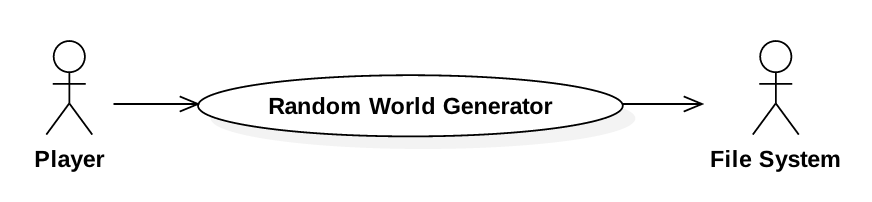
\includegraphics[width=0.4\textwidth]{diagrams/use-case-2-generate-random-world.png}
\end{center}

\begin{longtable}[c]{@{}p{0.2\textwidth}p{0.7\textwidth}@{}}
\toprule
& Ant Game: Generate Random World\tabularnewline
\midrule

Actors & A player, before a game or tournament.
Filesystem.\tabularnewline
Description & A tournament requires a world that conforms to the
specifications laid out in the functional requirements (see requirement
\texttt{World/2}). This component of the system can be interacted with
by the user to write a random world to file which conforms to these
specifications.\tabularnewline
Data & -\tabularnewline
Stimulus & Triggered by the user by interacting with the GUI, selecting
the option to generate a random ant world.\tabularnewline
Response & Generates a random ant world. Converts the ant world to a
textual description, as per functional requirement
\texttt{Parsing\ Specifications/World}. Asks the user where to save to
on disk, and then writes to a text file at that location.\tabularnewline
\bottomrule
\end{longtable}

\subsubsection{Upload Ant World}\label{upload-ant-world}

\begin{center}
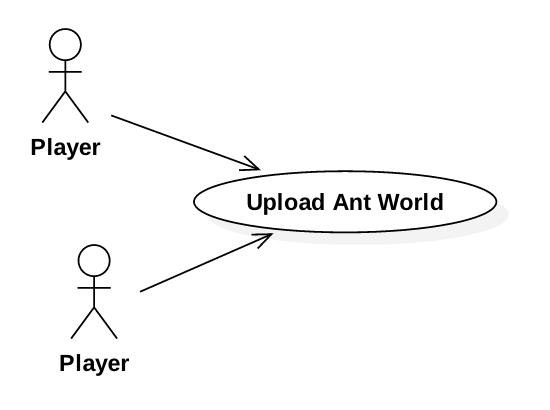
\includegraphics[width=0.4\textwidth]{diagrams/use-case-3-upload-ant-world.png}
\end{center}

\begin{longtable}[c]{@{}p{0.2\textwidth}p{0.7\textwidth}@{}}
\toprule
& Ant Game: Upload Ant World\tabularnewline
\midrule

Actors & Two or more players who agree to upload a particular ant world
to compete on.\tabularnewline
Description & In order to simulate a game or tournament, there must be
at least one ant world for the ants to compete on. These must be parsed
from file into memory.\tabularnewline
Data & The location of a file on disk.\tabularnewline
Stimulus & On the game and tournament setup screens, there will be a
button to upload an ant world. Once the user clicks on this, chooses a
file to parse, and clicks `Parse', this use case will be
invoked.\tabularnewline
Response & Whether the file represented a valid ant world as per the
functional requirements for parsing given in
\texttt{Parsing\ Specifications/World}. In addition, if this use case is
invoked in the context of a tournament setup, the additional criteria
for a contest world shall be checked (see requirement
\texttt{World/2}).\tabularnewline
\bottomrule
\end{longtable}

\subsubsection{Simulate Two Player Game}\label{simulate-two-player-game}

\begin{center}
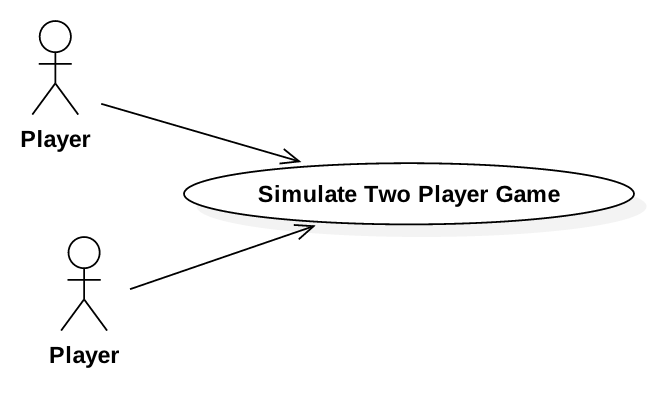
\includegraphics[width=0.4\textwidth]{diagrams/use-case-4-two-player-game.png}
\end{center}

\begin{longtable}[c]{@{}p{0.2\textwidth}p{0.7\textwidth}@{}}
\toprule
& Ant Game: Simulate Two Player Game\tabularnewline
\midrule

Actors & Two players.\tabularnewline
Description & Once the game setup is complete (with players setting the
ant brains and ant world) this use case comes next, with a competition
between the ants on the world being simulated.\tabularnewline
Data & The contextual data from other use cases will be in memory - the
world and brains. Some other relevant data shall be provided by the
user, such as the team names and options for game viewing (detailed in
the interface design section).\tabularnewline
Stimulus & The `Play' button on the game setup screen.\tabularnewline
Response & The system will simulate a game between the two ant colonies
as described in the functional requirements (\texttt{Game/1}). It will
present a simulation of the world as the ants carry out their actions.
At the end of the simulation, it will display the winner of the game to
the players, as well as relevant game statistics.\tabularnewline
\bottomrule
\end{longtable}

\subsubsection{Tournament}\label{tournament}

\begin{center}
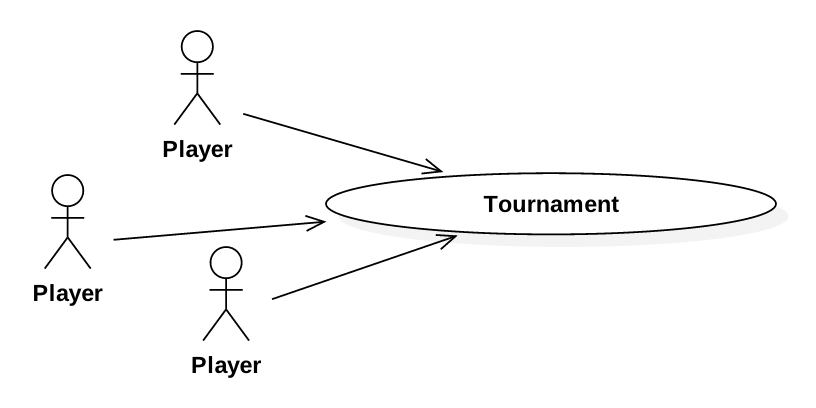
\includegraphics[width=0.4\textwidth]{diagrams/use-case-5-tournament.png}
\end{center}

\begin{longtable}[c]{@{}p{0.2\textwidth}p{0.7\textwidth}@{}}
\toprule
& Ant Game: Tournament\tabularnewline
\midrule

Actors & Two or more players.\tabularnewline
Description & This use case can be considered a `superset' of the use
Two Player Game use case. Once each of the players have uploaded the ant
brains and ant worlds, they can start a tournament to compete amongst
multiple ant brains on multiple ant worlds, to see which player is the
overall winner.\tabularnewline
Data & The contextual data from other use cases will be in memory - the
worlds (at least one, possibly several) and brains. As above, some other
relevant data shall be provided by the user, such as the team names and
options for game viewing.\tabularnewline
Stimulus & The `Play' button on the tournament setup
screen.\tabularnewline
Response & The system simulates an ant game between every possible
combination of teams, worlds, and colours (red or black). Then it
returns the final results of the tournament to the user (as per the
functional requirement \texttt{Game/3}) as well as statistics on the
game.\tabularnewline
\bottomrule
\end{longtable}

\subsection{System Components}\label{system-components}

From the functional requirements, the process model and use cases, the
main system components and their interactions have been modelled below.

\begin{center}
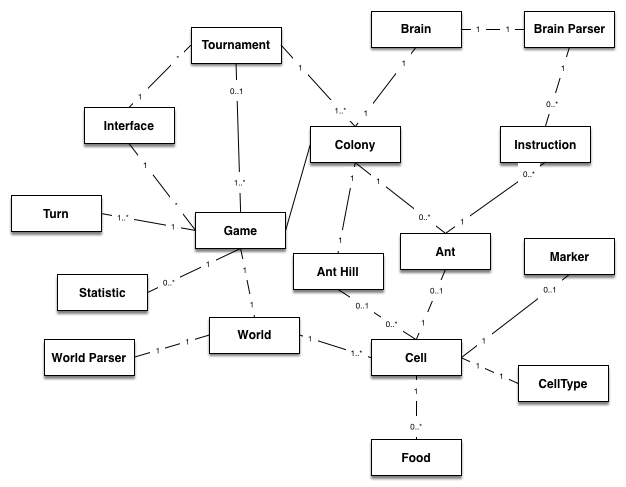
\includegraphics[width=\textwidth]{diagrams/system-components.png}
\end{center}

The system components diagram is extremely useful in terms of developing
a full design, and is the fundamental building block of the low-level
design section.

\newpage
\section{Low-Level}

\end{document}
